\documentclass[conference]{IEEEtran}
\IEEEoverridecommandlockouts
% The preceding line is only needed to identify funding in the first footnote. If that is unneeded, please comment it out.
\usepackage{cite}
\usepackage{amsmath,amssymb,amsfonts}
\usepackage{algorithmic}
\usepackage{graphicx}
\usepackage{textcomp}
\usepackage{xcolor}
\usepackage[brazilian]{babel}
\usepackage[utf8]{inputenc}
\usepackage[T1]{fontenc}
\usepackage{listings}
\usepackage{color}
\usepackage{float}
\usepackage{multirow}
\usepackage{hyperref}

\definecolor{dkgreen}{rgb}{0,0.6,0}
\definecolor{gray}{rgb}{0.5,0.5,0.5}
\definecolor{mauve}{rgb}{0.58,0,0.82}

\lstset{frame=tb,
  language=Java,
  aboveskip=3mm,
  belowskip=3mm,
  showstringspaces=false,
  columns=flexible,
  basicstyle={\small\ttfamily},
  numbers=none,
  numberstyle=\tiny\color{gray},
  keywordstyle=\color{blue},
  commentstyle=\color{dkgreen},
  stringstyle=\color{mauve},
  breaklines=true,
  breakatwhitespace=true,
  tabsize=3
}
\lstset{language=Python}
\def\BibTeX{{\rm B\kern-.05em{\sc i\kern-.025em b}\kern-.08em
    T\kern-.1667em\lower.7ex\hbox{E}\kern-.125emX}}
\begin{document}

\title{Relatório do Laboratório 12: \\ Aprendizado por Reforço Livre de Modelo\\
}

\author{\IEEEauthorblockN{Isabelle Ferreira de Oliveira}
\IEEEauthorblockA{\textit{CT-213 - Engenharia da Computação 2020} \\
\textit{Instituto Tecnológico de Aeronáutica (ITA)}\\
São José dos Campos, Brasil \\
isabelle.ferreira3000@gmail.com}
}

\maketitle

\begin{abstract}
Esse relatório documenta a implementação de algoritmos de Aprendizado por Reforço (RL) Livre de Modelo, a saber Sarsa e Q-Learning, e utilizá-los para resolver o problema do robô seguidor de linha.
\end{abstract}

\begin{IEEEkeywords}
Aprendizado por reforço, Sarsa, Q-Learning
\end{IEEEkeywords}

\section{Implementação}

\subsection{Implementação dos algoritmos de RL}

\subsubsection{Função epsilon\underline{\space}greedy\underline{\space}action}

A política epsilon-greedy foi implementada da seguinte maneira: gerou-se um número aleatório entre 0 e 1 e, caso esse valor aleatório seja menor que epsilon, então uma ação aleatória é escolhida; caso contrário, é escolhida a ação gulosa, através da chamada de greedy\underline{\space}action. 

\subsubsection{Função greedy\underline{\space}action}

Conforme sugerido na seção Dicas do roteiro \cite{roteiro}, foi pegue o índice do máximo elemento do array q[state], que é a tabela action-value para o estado naquele momento, e foi retornado esse valor.

\subsubsection{Função get\underline{\space}greedy\underline{\space}action para algoritmo Sarsa}

Retorna a função epsilon\underline{\space}greedy\underline{\space}action, aplicada na tabela action-value q, no estado em questão e com o episolon especificado.

\subsubsection{Função learn para algoritmo Sarsa} \label{learn_sarsa}

O aprendizado é feito atualizando o valor da tabela de action-value, acrescentando ao valor anterior o resultado de $ \alpha * (recompensa + \gamma * q[next state][next action] - q[state][action])$.

\subsubsection{Função get\underline{\space}greedy\underline{\space}action para algoritmo Q-Learning}

Retorna a função greedy\underline{\space}action, aplicada na tabela action-value q e no estado em questão.

\subsubsection{Função learn para algoritmo Q-learning}

Foi feito de forma análoga ao descrito em Função learn para algortimo Sarsa, \ref{learn_sarsa}.

\subsection{Aprendizado da política do robô seguidor de linha}

Para realizar o aprendizado do robô seguidor de linha, utilizando as duas técnicas implementadas anteriormente (Sarsa e Q-Learning), foi executado o script main.py, alterando-se o valor da variável rl\underline{\space}algorithm, entre os construtores: Sarsa e QLearning, com seus respectivos parâmetros.

\section{Resultados e Conclusões}

\subsection{Implementação dos algoritmos de RL}

Conforme apresentado nas Figuras \ref{sarsa_test_rl} e \ref{qlearning_test_rl}, pode-se observar resultados equivalentes para ambas as técnicas. Assim, tanto a tabela de action-value possuiu valores similares, como as sequências de ações foram idênticas nas duas situações.

\begin{figure}[htbp]
\centering
\centerline{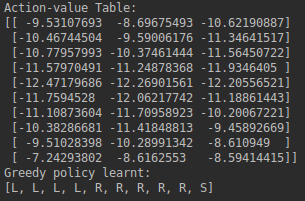
\includegraphics[scale=0.5]{imagens/sarsa_test_rl.png}}
\caption{Resultado obtido para algoritmo Sarsa, para tabela action-value e a sequência de ações.}.
\label{sarsa_test_rl}
\end{figure}

\begin{figure}[htbp]
\centering
\centerline{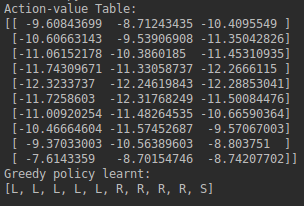
\includegraphics[scale=0.5]{imagens/qlearning_test_rl.png}}
\caption{Resultado obtido para algoritmo Q-Learning, para tabela action-value e a sequência de ações.}.
\label{qlearning_test_rl}
\end{figure} 

\subsection{Aprendizado da política do robô seguidor de linha}

Os resultados do aprendizado da política do robô seguidor de linha, utilizando os algoritmos de Sarsa e Q-Learning estão representados nas Figuras de \ref{sarsa/action_value_table} a \ref{sarsa/line_follower_solution} e \ref{q-learning/action_value_table} a \ref{q-learning/line_follower_solution}, respectivamente. 

\begin{figure}[htbp]
\centering
\centerline{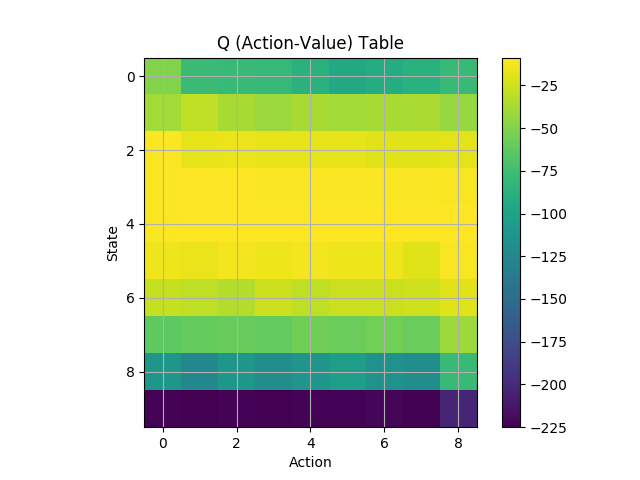
\includegraphics[scale=0.5]{imagens/sarsa/action_value_table.png}}
\caption{Representação em cores da tabela de action-value calculada, para algoritmo de Sarsa.}.
\label{sarsa/action_value_table}
\end{figure}

\begin{figure}[htbp]
\centering
\centerline{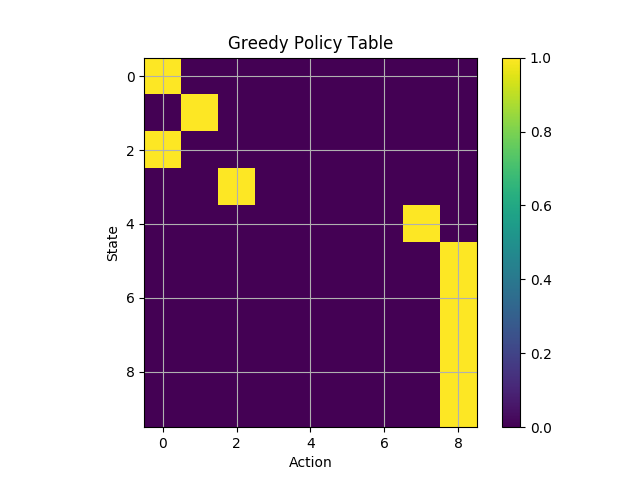
\includegraphics[scale=0.5]{imagens/sarsa/greedy_policy_table.png}}
\caption{Representação em cores da tabela de greedy-policy calculada, para algoritmo de Sarsa.}.
\label{sarsa/greedy_policy_table}
\end{figure} 

\begin{figure}[htbp]
\centering
\centerline{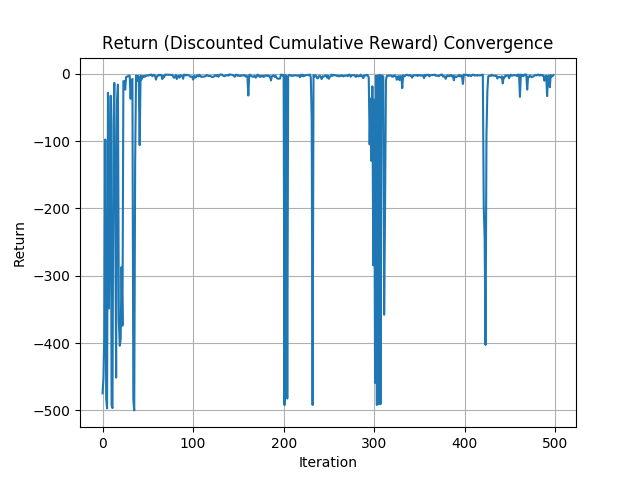
\includegraphics[scale=0.5]{imagens/sarsa/return_convergence.png}}
\caption{Recompensa acumulada em função das iterações, para algoritmo de Sarsa.}.
\label{sarsa/return_convergence}
\end{figure}

\begin{figure}[htbp]
\centering
\centerline{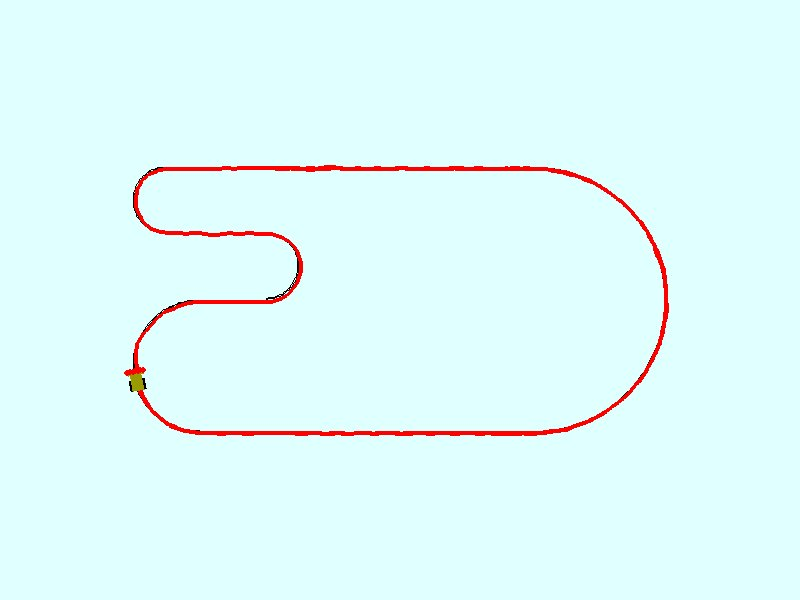
\includegraphics[scale=0.25]{imagens/sarsa/line_follower_solution.jpeg}}
\caption{Percurso aprendido pelo algoritmo de Sarsa.}.
\label{sarsa/line_follower_solution}
\end{figure}

bçabjfjfça

\begin{figure}[htbp]
\centering
\centerline{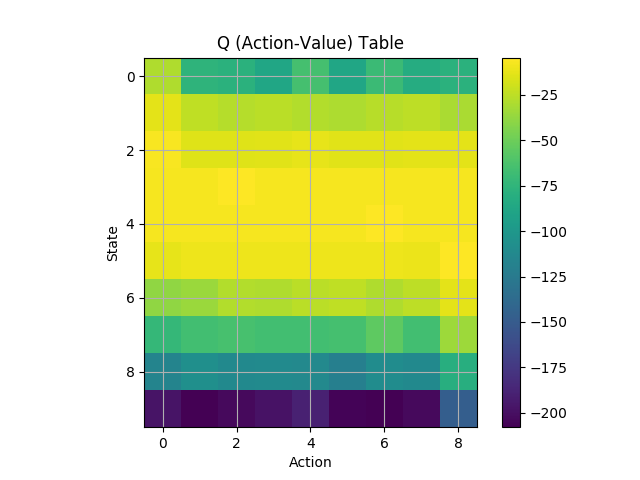
\includegraphics[scale=0.5]{imagens/q-learning/action_value_table.png}}
\caption{Representação em cores da tabela de action-value calculada, para algoritmo de Q-Learning.}.
\label{q-learning/action_value_table}
\end{figure}

\begin{figure}[htbp]
\centering
\centerline{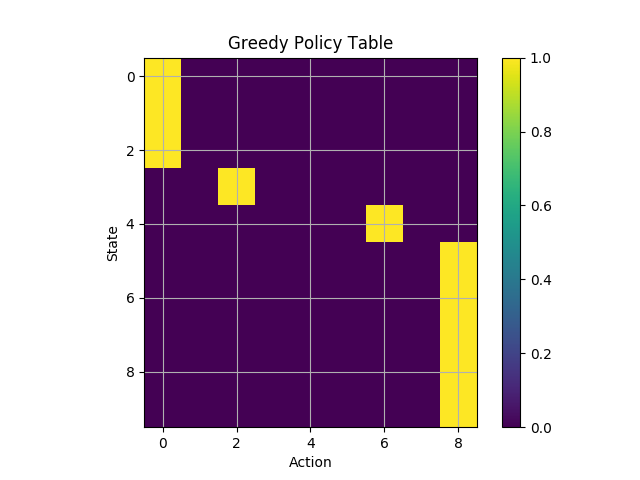
\includegraphics[scale=0.5]{imagens/q-learning/greedy_policy_table.png}}
\caption{Representação em cores da tabela de greedy-policy calculada, para algoritmo de Q-Learning.}.
\label{q-learning/greedy_policy_table}
\end{figure}

\begin{figure}[htbp]
\centering
\centerline{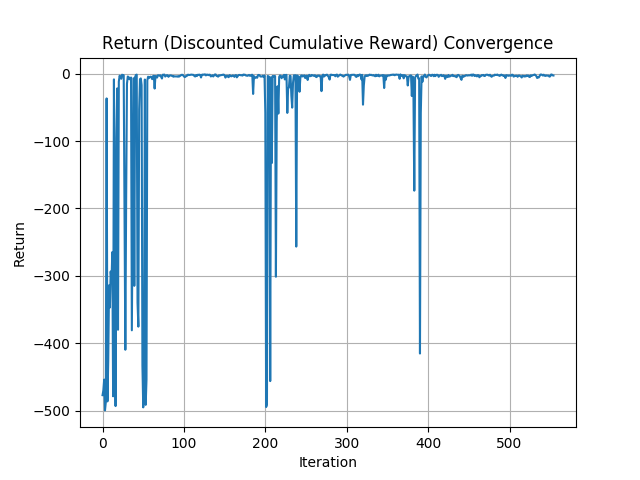
\includegraphics[scale=0.5]{imagens/q-learning/return_convergence.png}}
\caption{Recompensa acumulada em função das iterações, para algoritmo de Q-Learning.}.
\label{q-learning/return_convergence}
\end{figure}

\begin{figure}[htbp]
\centering
\centerline{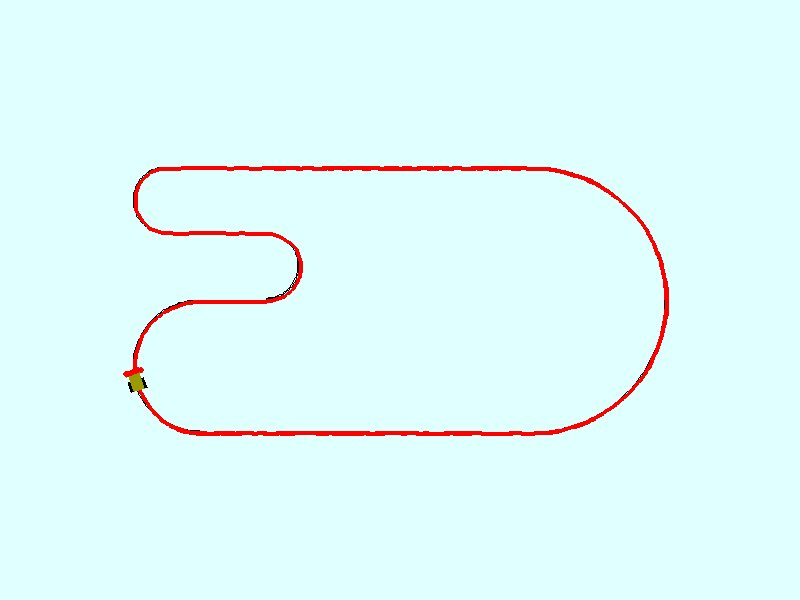
\includegraphics[scale=0.25]{imagens/q-learning/line_follower_solution.jpeg}}
\caption{Percurso aprendido pelo algoritmo de Q-Learning.}.
\label{q-learning/line_follower_solution}
\end{figure}

\begin{enumerate}
\item CORRECT\underline{\space}ACTION\underline{\space}PROB = 0.8

\item GAMMA = 0.98
\end{enumerate}

Primeiro comparando-se os resultados apresentados nas Figuras \ref{grid2/value_iteration} e \ref{grid2/policy_iteration}, também é possível notar que eles são idênticos, o que é novamente esperado, uma vez que ambas as técnicas levam a convergência dos valores corretos de \textit{policy} e \textit{value}.

Sobre a Figura \ref{grid2/policy_evaluation}, a mesma tendência que no primeiro Grid World é observada, ou seja, o \textit{value} calculado é maior em módulo para estados mais distantes do estado objetivo.

Nos três resultados também é possível notar o \textit{value} 0.0 para o estado objetivo, o que também condiz com o esperado. 

Por fim, comparando-se as duas situações de Grid World, é possível notar que, com a adição do desconto \textit{GAMMA}, e agora com a probabilidade de o agente executar uma ação diferente da escolhida para cada estado, tem-se que os \textit{value} referentes a cada estado são maiores em módulo do que os calculados na primeira situação.

Isso se justifica e condiz com o esperado, uma vez que não se sabendo deterministicamente a ação tomada em cada estado, a função valor entende esse estado como "pior" quando comparado a situação na qual \textit{CORRECT\underline{\space}ACTION\underline{\space}PROB} = 1. Além disso, o fator \textit{GAMMA} adiciona mais imediatismo à recompensa das ações do agente, o que também diminui a medida de quão "bom" é determinado estado em comparação a situação no qual todas as recompensas até o objetivo são igualmente contabilizadas.

\begin{thebibliography}{00}
\bibitem{roteiro} M. Maximo, ``Roteiro: Laboratório 11 - Programação Dinâmica''. Instituto Tecnológico de Aeronáutica, Departamento de Computação. CT-213, 2019.
\end{thebibliography}

\end{document}
